\PassOptionsToPackage{table}{xcolor}
\documentclass[12pt,letterpaper,twocolumn,openany,nodeprecatedcode,bg=none]{dndbook}
\usepackage[english]{babel}
\usepackage[utf8]{inputenc}
\usepackage{longtable,booktabs,array}
\usepackage{calc}
\usepackage{etoolbox}
\usepackage{caption}
\usepackage{float}
\usepackage{graphicx}
\usepackage{needspace}
\usepackage{tikz}

% Reset zebra striping at the start of every table
\AtBeginEnvironment{longtable}{\rowcolors{1}{white}{gray!10}\small}
\AtBeginEnvironment{table}{\rowcolors{1}{white}{gray!10}}

\providecommand{\pandocbounded}[1]{#1}
\providecommand{\tightlist}{%
  \setlength{\itemsep}{0pt}\setlength{\parskip}{0pt}}

\captionsetup{labelformat=empty}
\setcounter{secnumdepth}{0}
\setlength{\parindent}{0pt}
\setlength{\parskip}{0.5\baselineskip}
\setlength{\headheight}{15pt}

% Prevent orphaned subsections
\let\oldsubsection\subsection
\renewcommand{\subsection}[1]{%
  \needspace{5\baselineskip}%
  \oldsubsection{#1}%
}

\begin{document}
\onecolumn

      \title{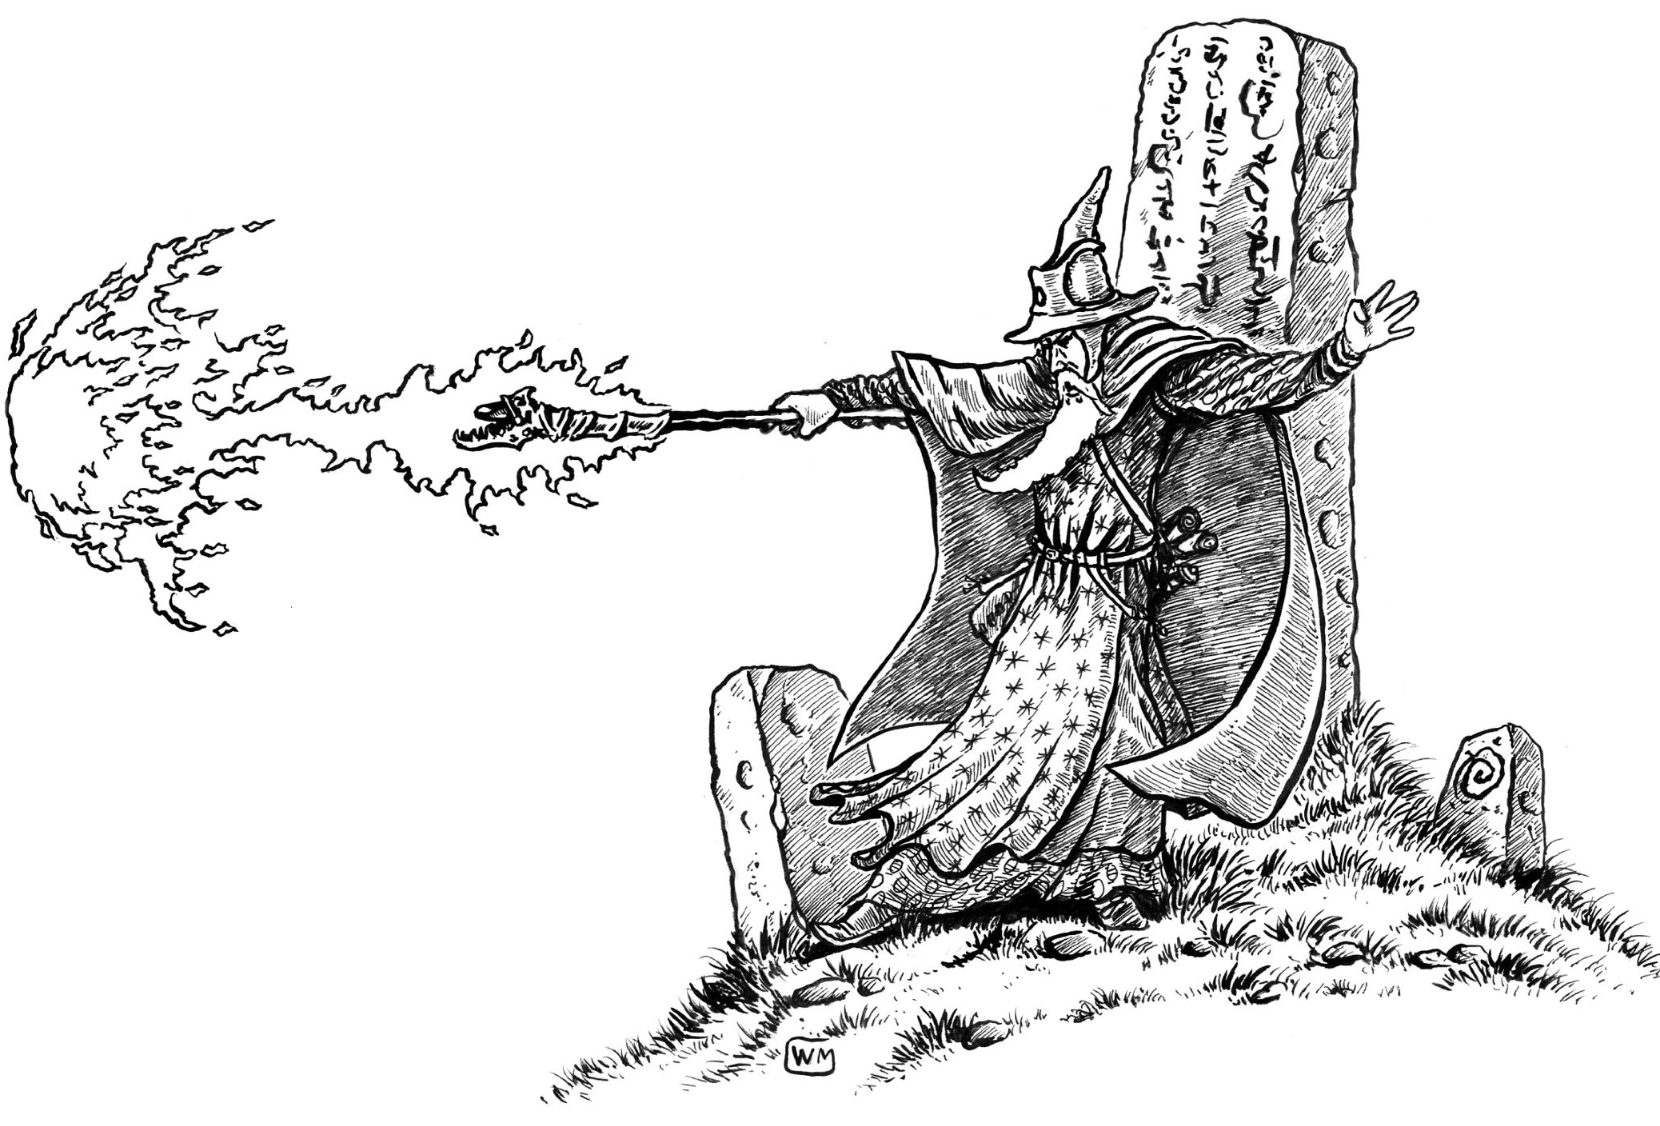
\includegraphics[width=0.9\textwidth,height=0.55\textheight,keepaspectratio]{classicWizard.png}\\[1.5cm]Wizard}
  \author{Class Handbook}
\date{}
\maketitle

\clearpage
\thispagestyle{empty}
\null\vfill
\begin{center}{\Large\itshape Your trusty class handbook for fantasy
gaming.}\end{center}
\vfill

\clearpage
\thispagestyle{empty}
\begin{center}
\vspace*{\fill}
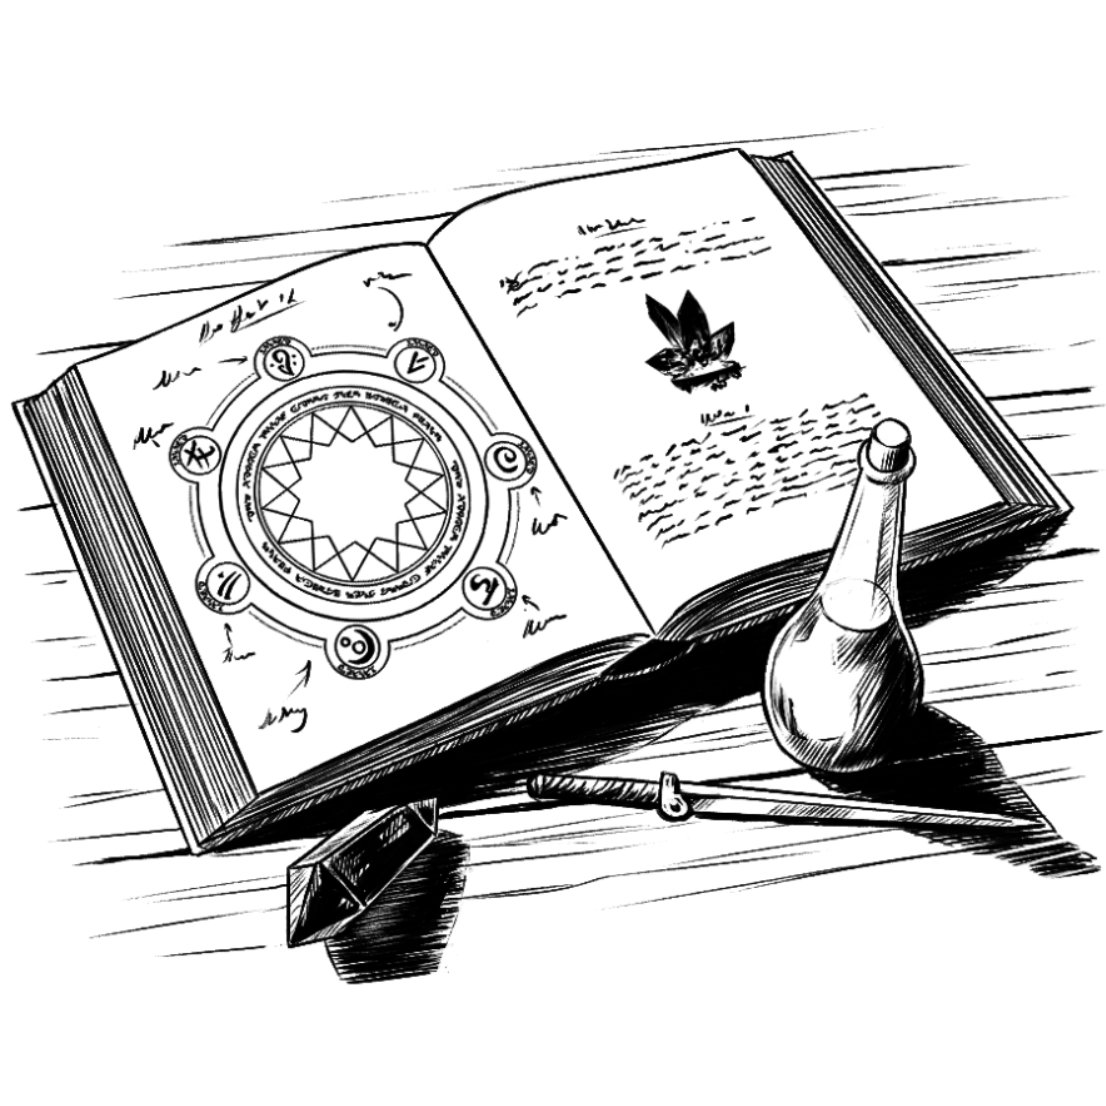
\includegraphics[width=\textwidth,height=0.85\textheight,keepaspectratio]{spellbook.png}\par
\vspace{0.4cm}
{\itshape Every wizard needs a spellbook.}\par
\vspace*{\fill}
\end{center}

\clearpage
\twocolumn

\section{Wizard}\label{wizard}

\subsection{Core Wizard Traits}\label{core-wizard-traits}

{\def\LTcaptype{none} % do not increment counter
\begin{table}[H]
\centering
\begin{tabular}{@{}
  >{\raggedright\arraybackslash}p{(\linewidth - 2\tabcolsep) * \real{0.4478}}
  >{\raggedright\arraybackslash}p{(\linewidth - 2\tabcolsep) * \real{0.5522}}@{}}
\toprule\noalign{}
\begin{minipage}[b]{\linewidth}\raggedright
\textbf{Primary Ability}
\end{minipage} & \begin{minipage}[b]{\linewidth}\raggedright
Intelligence
\end{minipage} \\
\midrule\noalign{}
\textbf{Hit Points} & 1d4 \\
\textbf{Saving Throw Proficiencies} & Intelligence, Wisdom \\
\textbf{Skill Proficiencies} & Choose 2 skills \\
\textbf{Weapon Proficiencies} & Choose 1 category \\
\textbf{Starting Equipment} & Padded Jacket, Staff, Spellbook, Robe \\
\bottomrule\noalign{}
\end{tabular}
\end{table}
}

\subsection{Wizard Features}\label{wizard-features}

{\def\LTcaptype{none} % do not increment counter
\begin{table}[H]
\centering
\begin{tabular}{@{}lll@{}}
\toprule\noalign{}
Level & Proficiency & Class Features \\
\midrule\noalign{}
1 & +2 & Spellcasting \\
2 & +2 & --- \\
3 & +2 & Ability Bonus \\
4 & +2 & --- \\
5 & +2 & --- \\
6 & +2 & --- \\
7 & +2 & Ability Bonus \\
8 & +2 & --- \\
9 & +3 & --- \\
10 & +3 & --- \\
\bottomrule\noalign{}
\end{tabular}
\end{table}
}

\subsection{Level 1: Spellcasting}\label{level-1-spellcasting}

You can cast spells from the Wizard spell list. Intelligence is your
casting ability. You know two cantrips.

You have a spellbook that contains all your known spells. You start with
three level 1 spells. You add another spell to your book each time you
gain a level.

You regain all expended spell slots when you finish a long rest. Once
per day, you may regain 1 expended spell slot when you finish a short
rest.

\subsection{Spell Slots by Level}\label{spell-slots-by-level}

{\def\LTcaptype{none} % do not increment counter
\begin{table}[H]
\centering
\begin{tabular}{@{}llll@{}}
\toprule\noalign{}
Level & 1 & 2 & 3 \\
\midrule\noalign{}
1 & 2 & -- & -- \\
2 & 2 & -- & -- \\
3 & 3 & -- & -- \\
4 & 3 & -- & -- \\
5 & 4 & 2 & -- \\
6 & 4 & 2 & -- \\
7 & 4 & 3 & -- \\
8 & 4 & 3 & -- \\
9 & 4 & 3 & 2 \\
10 & 4 & 3 & 2 \\
\bottomrule\noalign{}
\end{tabular}
\end{table}
}

\subsection{Level 3: Ability Bonus}\label{level-3-ability-bonus}

You gain a +1 bonus to two different abilities of your choice.

\subsection{Level 7: Ability Bonus}\label{level-7-ability-bonus}

You gain a +1 bonus to two different abilities of your choice.

\subsection{Wizard Spells}\label{wizard-spells}

The tables are numbered to allow quick generation of spells known for a
new character.

\subsubsection{Cantrips}\label{cantrips}

{\def\LTcaptype{none} % do not increment counter
\begin{table}[H]
\centering
\begin{tabular}{@{}ll@{}}
\toprule\noalign{}
d6 & Cantrip \\
\midrule\noalign{}
1 & Fire Bolt \\
2 & Light \\
3 & Mage Hand \\
4 & Minor Illusion \\
5 & Prestidigitation \\
6 & Ray of Frost \\
\bottomrule\noalign{}
\end{tabular}
\end{table}
}

\subsubsection{Level 1 Spells}\label{level-1-spells}

{\def\LTcaptype{none} % do not increment counter
\begin{table}[H]
\centering
\begin{tabular}{@{}ll@{}}
\toprule\noalign{}
d10 & Level 1 \\
\midrule\noalign{}
1 & Alarm \\
2 & Burning Hands \\
3 & Comprehend Languages \\
4 & Detect Magic \\
5 & Disguise Self \\
6 & Feather Fall \\
7 & Grease \\
8 & Mage Armor \\
9 & Magic Missile \\
10 & Thunderwave \\
\bottomrule\noalign{}
\end{tabular}
\end{table}
}

\subsubsection{Level 2 Spells}\label{level-2-spells}

{\def\LTcaptype{none} % do not increment counter
\begin{table}[H]
\centering
\begin{tabular}{@{}ll@{}}
\toprule\noalign{}
d8 & Level 2 \\
\midrule\noalign{}
1 & Darkness \\
2 & Detect Thoughts \\
3 & Invisibility \\
4 & Levitate \\
5 & Mirror Image \\
6 & Misty Step \\
7 & Scorching Ray \\
8 & See Invisibility \\
\bottomrule\noalign{}
\end{tabular}
\end{table}
}

\subsubsection{Level 3 Spells}\label{level-3-spells}

{\def\LTcaptype{none} % do not increment counter
\begin{table}[H]
\centering
\begin{tabular}{@{}ll@{}}
\toprule\noalign{}
d8 & Level 3 \\
\midrule\noalign{}
1 & Dispel Magic \\
2 & Fear \\
3 & Fireball \\
4 & Fly \\
5 & Haste \\
6 & Lightning Bolt \\
7 & Speak with Dead \\
8 & Water Breathing \\
\bottomrule\noalign{}
\end{tabular}
\end{table}
}

\pagebreak

\section{Wizard Spell List}\label{wizard-spell-list}

Spells descriptions are listed below.

\subsection{Alarm}\label{alarm}

\textbf{Level:} 1

\textbf{Range:} 30 feet

\textbf{Duration:} 8 hours

You set an alarm against intrusion. Choose a door, a window, or an area
within range that is no larger than a 20-foot cube. An alarm alerts you
whenever a creature touches or enters the warded area. When you cast the
spell, you can designate creatures that won't set off the alarm. You
also choose whether the alarm is audible or mental:

\textbf{Audible Alarm.} The alarm produces the sound of a handbell for
10 seconds within 60 feet of the warded area.

\textbf{Mental Alarm.} You are alerted by a mental ping if you are
within 1 mile of the warded area. This ping awakens you if you're
asleep.

\subsection{Burning Hands}\label{burning-hands}

\textbf{Level:} 1

\textbf{Range:} Self

A thin sheet of flames shoots forth from you. Each creature in a 15-foot
cone projected from you makes a Dexterity saving throw, taking 3d6 fire
damage on a failed save or half damage on a successful one.

The damage increases to 5d6 fire damage if you use a level 2 slot and
7d6 fire damage if you use a level 3 slot.

\subsection{Comprehend Languages}\label{comprehend-languages}

\textbf{Level:} 1

\textbf{Range:} Touch

\textbf{Duration:} 1 hour

Your magic aligns a creature's mind with pure magical thought, allowing
it to communicate with any creature. The creature you touch can
understand any spoken or signed language that it hears or sees, and its
speech or gestures are understood by any creature that has a language.

\subsection{Darkness}\label{darkness}

\textbf{Level:} 2

\textbf{Range:} 60 feet

\textbf{Duration:} Concentration, up to 10 minutes

Darkness spreads from a point within range and fills a 15-foot-radius
sphere.

Darkvision can't see through it, and nonmagical light can't illuminate
it. Magical sources of light created by level 2 or lower spells shed no
light in this area.

\subsection{Detect Magic}\label{detect-magic}

\textbf{Level:} 1

\textbf{Range:} Self

\textbf{Duration:} Concentration, up to 10 minutes

You see the presence of magical effects within 30 feet on objects that
are visible to you. Magic appears as a faint aura, the details of which
allow you to determine its origin and the basic details of its effect.

\subsection{Detect Thoughts}\label{detect-thoughts}

\textbf{Level:} 2

\textbf{Range:} Self

\textbf{Duration:} Concentration, up to 1 minute

You sense the presence of thoughts within 30 feet that belong to
creatures that know languages or are telepathic.

You don't read the thoughts, but you know that a thinking creature is
present.

The spell is blocked by 1 inch of solid material.

If you can see a creature, as an action or when you cast this spell you
can force it to make a Wisdom save. If it fails, you search its thoughts
and learn the answer to one question you ask it. You learn the truth as
the creature understands it. If it succeeds, the spell ends.

\subsection{Disguise Self}\label{disguise-self}

\textbf{Level:} 1

\textbf{Range:} Self

\textbf{Duration:} 1 hour

You make yourself, including your belongings, look different. You can
seem 1 foot shorter or taller and can appear heavier or lighter.

The changes wrought by this spell fail to hold up to physical
inspection.

An observer can notice this is an illusion with a successful
Intelligence (Investigation) check against your spell save DC.

\subsection{Dispel Magic}\label{dispel-magic}

\textbf{Level:} 3

\textbf{Range:} 120 feet

Choose one creature, object, or magical effect within range. Any ongoing
spell of level 3 or lower on the target ends. For each ongoing spell of
level 4 or higher on the target, make an ability check using your
spellcasting ability (DC 10 plus that spell's level). On a successful
check, the spell ends.

\subsection{Fear}\label{fear}

\textbf{Level:} 3

\textbf{Range:} Self

\textbf{Duration:} Concentration, up to 1 minute

Each creature in a 30-foot cone projected from you must succeed on a
Wisdom saving throw or drop whatever it is holding and become frightened
of you for the duration.

If the creature ends its turn in a space where it doesn't have line of
sight to you, the creature makes a Wisdom saving throw. On a successful
save, the spell ends on that creature.

\subsection{Feather Fall}\label{feather-fall}

\textbf{Level:} 1

\textbf{Range:} 60 feet

\textbf{Duration:} 1 minute

You can cast this spell in response to falling or seeing someone fall.
Choose up to five falling creatures within range. A falling creature's
rate of descent slows to 60 feet per round. If a creature lands before
the spell ends, the creature takes no damage from the fall, and the
spell ends for that creature.

\subsection{Fireball}\label{fireball}

\textbf{Level:} 3

\textbf{Range:} 150 feet

A bright streak flashes from you to a point you choose within range and
then blossoms with a low roar into a fiery explosion. Each creature in a
20-foot-radius sphere centered on that point makes a Dexterity saving
throw, taking 8d6 fire damage on a failed save or half damage on a
successful one.

\subsection{Fire Bolt}\label{fire-bolt}

\textbf{Level:} Cantrip

\textbf{Range:} 120 feet

You hurl a mote of fire at a target within range. Make a ranged attack
against the target. On a hit, the target takes 1d10 fire damage.

The damage increases to 2d10 fire damage at level 5 and 3d10 fire damage
at level 9.

\subsection{Fly}\label{fly}

\textbf{Level:} 3

\textbf{Range:} Touch

\textbf{Duration:} Concentration, up to 10 minutes

You touch a willing creature. For the duration, the target gains a fly
speed.

When the spell ends, the target falls if it is still aloft unless it can
stop the fall.

\subsection{Grease}\label{grease}

\textbf{Level:} 1

\textbf{Range:} 60 feet

\textbf{Duration:} 1 minute

Grease covers the ground in a 10-foot square centered on a point within
range.

When the grease appears, each creature standing in its area must succeed
on a Dexterity saving throw or fall prone. A creature that moves into or
in area or ends its turn there must also succeed on that save or fall
prone. A creature need only make this save once per turn.

\subsection{Haste}\label{haste}

\textbf{Level:} 3

\textbf{Range:} 30 feet

\textbf{Duration:} Concentration, up to 1 minute

Choose a willing creature within range. On each of its turns, it can
choose to take a second action. If it does so, roll a d20. On an 11 or
higher, it gains a failed death save.

\subsection{Invisibility}\label{invisibility}

\textbf{Level:} 2

\textbf{Range:} Touch

\textbf{Duration:} Concentration, up to 1 hour

A creature you touch becomes invisible. The spell ends early immediately
after the target makes an attack roll, deals damage, or casts a spell.

If you cast this spell with a level 3 slot, you can target two
creatures.

\subsection{Levitate}\label{levitate}

\textbf{Level:} 2

\textbf{Range:} 60 feet

\textbf{Duration:} Concentration, up to 10 minutes

One creature or loose object of your choice within range rises
vertically up to 20 feet and remains suspended there. The spell can
levitate an object that weighs up to 500 pounds. An unwilling creature
that succeeds on a Constitution saving throw is unaffected.

The target can move only by pushing or pulling against a fixed object or
surface within reach (such as a wall or a ceiling), which allows it to
move as if it were climbing. You can change the target's altitude by up
to 20 feet in either direction on your turn. If you are the target, you
can move up or down as part of your move. Otherwise, you can take an
action to move the target, which must remain within the spell's range.

When the spell ends, the target floats gently to the ground if it is
still aloft.

\subsection{Light}\label{light}

\textbf{Level:} Cantrip

\textbf{Range:} Touch

\textbf{Duration:} 1 hour

An object you touch sheds dim light in a 30-foot radius and Dim Light
for an additional 20 feet. The spell ends if you cast it again.

\subsection{Lightning Bolt}\label{lightning-bolt}

\textbf{Level:} 3

\textbf{Range:} 300 feet

You can make ranged spell attacks against up to three targets. The
damage is 6d10 lightning damage if you attack three targets, 8d10
lightning damage if you attack two, or 10d10 lightning damage if you
attack one. If the attack misses, the target takes half damage.

\subsection{Mage Armor}\label{mage-armor}

\textbf{Level:} 1

\textbf{Range:} Touch

\textbf{Duration:} 8 hours

You touch a creature. Until the spell ends, the target can treat its AC
as 13 + its Dexterity modifier.

\subsection{Mage Hand}\label{mage-hand}

\textbf{Level:} Cantrip

\textbf{Range:} 30 feet

\textbf{Duration:} 1 minute

A spectral, floating hand appears at a point you choose within range.
The hand vanishes if it is ever more than 30 feet away from you or if
you cast this spell again.

When you cast the spell, you can use the hand to manipulate an object,
open an unlocked door or container, stow or retrieve an item from an
open container, or pour the contents out of a vial.

As an action on your later turns, you can control the hand thus again.
As part of that action, you can move the hand up to 30 feet.

The hand can't attack, activate magic items, or carry more than 10
pounds.

\subsection{Magic Missile}\label{magic-missile}

\textbf{Level:} 1

\textbf{Range:} 120 feet

You create three glowing darts of magical force. Each dart strikes a
creature of your choice that you can see within range. A dart deals 1d4
+ 1 force damage to its target.

The damage increases to 2d4 + 2 force damage if you use a level 2 slot
and 3d4 + 3 force damage if you use a level 3 slot.

\subsection{Minor Illusion}\label{minor-illusion}

\textbf{Level:} Cantrip

\textbf{Range:} 30 feet

\textbf{Duration:} 1 minute

You create a sound or an image of an object within range that lasts for
the duration. See the descriptions below for the effects of each. The
illusion ends if you cast this spell again.

A creature can determine that it is an illusion with a successful
Intelligence (Investigation) check against your spell save DC.

\textbf{Sound.} If you create a sound, its volume can range from a
whisper to a scream that can last up to the spell's duration.

\textbf{Image.} An image you create cannot be larger than a 5-foot cube
or a size Medium creature. The image can't create sound, light, smell,
or any other sensory effect. Physical interaction with the image reveals
it to be an illusion.

\subsection{Mirror Image}\label{mirror-image}

\textbf{Level:} 2

\textbf{Range:} Self

\textbf{Duration:} 1 minute

Three illusory duplicates of yourself appear in your space. The
duplicates move with you and mimic your actions, shifting position so
it's impossible to track which image is real.

Each time a creature hits you with an attack roll during the spell's
duration, roll a d6 for each of your remaining duplicates. If any of the
d6s rolls a 3 or higher, one of the duplicates is hit instead of you,
and the duplicate is destroyed. The duplicates otherwise ignore all
other damage and effects. The spell ends when all three duplicates are
destroyed.

A creature is unaffected by this spell if it cannot see or can use other
senses to pinpoint you.

\subsection{Misty Step}\label{misty-step}

\textbf{Level:} 2

\textbf{Range:} Self

Briefly surrounded by silvery mist, you teleport up to 30 feet to an
unoccupied space you can see. Casting this spell does not use your
action.

\subsection{Prestidigitation}\label{prestidigitation}

\textbf{Level:} Cantrip

\textbf{Range:} 10 feet

\textbf{Duration:} Up to 1 hour

You create a minor magical effect within range. You can light a torch,
create a glowing sigil, clean off an object, or create an object that
can fit in the palm of your hand. An object created in this manner is an
obvious, worthless duplicate. The spell ends if you cast it again.

\subsection{Ray of Frost}\label{ray-of-frost}

\textbf{Level:} Cantrip

\textbf{Range:} 60 feet

A frigid beam of blue-white light streaks toward a creature within
range. Make a ranged spell attack against the target. On a hit, it takes
1d8 cold damage, and its speed is reduced by 20 feet until after its
next turn.

The damage increases to 2d8 cold damage at level 5 and 3d8 cold damage
at level 9.

\subsection{Scorching Ray}\label{scorching-ray}

\textbf{Level:} 2

\textbf{Range:} 120 feet

You hurl three fiery rays. You can hurl them at one target within range
or at several. Make a ranged spell attack for each ray. On a hit, the
target takes 2d6 fire damage.

If you cast this spell with a level 3 slot, the damage increases to 3d6
fire damage.

\subsection{See Invisibility}\label{see-invisibility}

\textbf{Level:} 2

\textbf{Range:} Self

\textbf{Duration:} 1 hour

You see creatures and objects that are invisible as if they were
visible.

\subsection{Speak with Dead}\label{speak-with-dead}

\textbf{Level:} 3

\textbf{Range:} 10 feet

\textbf{Duration:} 10 minutes

You touch a corpse and attempt to commune with its spirit. If its spirit
can be contacted, you contact it through mystical means.

Until the spell ends, you can ask the spirit of the corpse up to five
questions. The spirit knows only what it knew in life, including the
languages it knew. The spirit is under no compulsion to offer a truthful
answer if you are antagonistic toward it or it recognizes you as an
enemy.

The dead often demand a service in return for the information they
provide. If you accept such a deal, you cannot cast this spell again
until you complete the task or make a good faith effort to do so.

\subsection{Thunderwave}\label{thunderwave}

\textbf{Level:} 1

\textbf{Range:} Self

You unleash a wave of thunderous energy. Each creature in a 15-foot cube
originating from you makes a Constitution saving throw. On a failed
save, a creature takes 2d8 thunder damage and is pushed 10 feet away
from you. On a successful save, a creature takes half damage.

Unsecured objects that are entirely within the cube are pushed 10 feet
away from you, and a thunderous boom is audible within 300 feet.

The damage increases to 3d8 thunder damage if you use a level 2 slot and
4d8 thunder damage if you use a level 3 slot.

\subsection{Water Breathing}\label{water-breathing}

\textbf{Level:} 3

\textbf{Range:} 30 feet

\textbf{Duration:} 24 hours

This spell grants up to ten willing creatures of your choice within
range the ability to breathe underwater until the spell ends. Affected
creatures also retain their normal mode of respiration.

\onecolumn

\clearpage
\thispagestyle{empty}
\begin{center}
\vspace*{\fill}

\includegraphics[width=0.7\textwidth,keepaspectratio]{magicBook.jpg}\par
\vspace{0.4cm}
{\itshape Does the wizard make the spellbook? Or does the spellbook make
the wizard?}\par
\vspace*{\fill}
\end{center}

\end{document}